\documentclass{deliverablereport}

% \usepackage[style=alphabetic,backend=bibtex]{biblatex}
\usepackage[style=ieee,backend=bibtex]{biblatex}
\addbibresource{report.bib}
\addbibresource{../../lib/publications.bib}

\usepackage{xparse}
\usepackage{etoolbox}
\usepackage{caption}

\deliverable{dissem}{oommfnb-vre-deliver}
\duedate{31/08/2018 (M48)}
\deliverydate{30/08/2019}
\author{Marijan Beg and Hans Fangohr}

\begin{document}
\maketitle
\githubissuedescription
\newpage
\tableofcontents
\newpage

\section{Introduction}
The primary focus of the \ODK project is to improve e-infrastructure
for research in mathematics and to provide a Jupyter project based
virtual research environment. However, significant parts of these
investments are of applicability to a much wider range of activities
outside mathematics research.

With this deliverable we want to demonstrate the power of the
(improved) Jupyter-based virtual research environment with application
in the computational magnetism research domain, as a representative of
the growing field of computational science and engineering.

In this deliverable report, we start by introducing the concept of
micromagnetics and the simulation tool OOMMF. After that, we present
the conventional computational workflow with OOMMF and identify its
disadvantages. Subsequently, the benefits of building a Python
interface to OOMMF and embedding simulations into Jupyter notebook are
stated. The rest of the report deals with the implementation details,
such as subpackages, code hosting, testing, continuous integration,
packaging, and documentation. Finally, we complete the report by
reporting the dissemination activities we conducted as well as the
evaluation data we collected.

\section{Introduction to Computational Micromagnetics}
\subsection{Computational Magnetism}

Magnetism underpins modern life through a number of technologies,
including magnetic data storage (disk and tape, used widely in the
service sector, Google, Netflix, Amazon, etc), magnetic sensors (for
example to monitor steering wheel positions or rotational velocity of
tires), magnetic resonance imaging in the medical sector, and
permanent magnets in electric cars.

Research in this field is increasingly enabled and underpinned by
computational approaches: often the appropriate equations (here time
dependent partial integro-differential equations) are known but
analytically impossible to solve. By discretising space and time (for
example using finite differences or finite elements), problems can be
computed for a particular set of initial conditions and boundary
conditions.

In the following, we focus on magnetism at the nanoscale -
this is technically known as micromagnetism - which is technologically
relevant for data storage, sensors, and potential new storage and
computing paradigms.



\subsection{Object Oriented MicroMagnetic Framework (OOMMF)}

The Object Oriented MicroMagnetic Framework (OOMMF)~\cite{Donahue1999}
is a micromagnetic simulation tool, for which development started
during the 1990s at the National Institute of Science and Technology
(NIST) by Michael Donahue and Don Porter. It is probably the most
widely used and most trusted simulation tool in the micromagnetic
scientific community, and still maintained and further developed. It
was written in C++ and wrapped with Tcl, which is the language that
must be used to configure simulations by the user.

\subsection{Original computational workflow}

The computational workflow that had to be done by the user in order to simulate a
particular micromagnetic problem was as follows:

\begin{enumerate}
\item A configuration script (\texttt{.mif}) file was written in Tcl,
  so that all characteristics of the micromagnetic system were
  specified (geometry, Hamiltonian, dynamics equation, initial
  configuration of magnetisation field, boundary conditions, etc.).
\item OOMMF was run by providing a configuration \texttt{.mif} file via
  Terminal/Command Prompt. After the OOMMF run was complete, the
  spatially resolved vector fields were saved as \texttt{.omf} files
  for many time steps and scalar data was saved in an \texttt{.odt}
  file.
\item If another run with different parameters was necessary steps 1
  and 2 are repeated.
\item Resulting files were opened and analysed by the user either using
  OOMMF and its GUI-driven tools or command line driven tools or
  different data analysis tools; typically by manually carrying out
  sequences of analysis steps.
\end{enumerate}

We want to address several issues that are related
to this particular type of workflow (which is found widely in
computational science):
\begin{itemize}
\item It is difficult for an average user to automate the process
of running many different simulations with different parameters.
\item It is difficult to keep a log of all steps performed in the
entire micromagnetic study.
\item Postprocessing and the analysis of results is performed outside
OOMMF using techniques and scripts developed by the user, or done manually.
\end{itemize}

All these issues compromise the reproducibility of the micromagnetic
study because it is very difficult to convey the exact simulation
procedure. They also reduce the effectiveness of the research: experts
in - for example - materials science and physics have to spend time to
execute computational commands repeatedly while changing parameters in
input files, then search for output files, and extract the new results
for the new parameter, etc.

\subsection{Workflow with Jupyter embedded research environment}

The main goal of this deliverable was
to develop a Micromagnetic Virtual Research Environment (VRE) which
would address this problem. More precisely, the goal was to develop a
Python interface to OOMMF and integrate it into Jupyter
notebook.

Benefits of this approach include:
\begin{itemize}
\item One document describes the whole study: Jupyter notebooks can
  contain (i) simulation and data analysis code, (ii) code output,
  such as numerical and visualised data, and (iii) human-readable
  text; see figure \ref{fig:demo1} on page \pageref{fig:demo1} for an example.
\item Improved reproducibility: all the necessary
information required to make the study reproducible are contained in a
single document which can be later shared, modified, and
re-executed.
\item Embedding the domain specific language (here scripting of
  computational micromagnetics) into Python provides a general purpose
  computing environment without having to invest new configuration
  file syntax and parses: For example, running different simulations
  with different parameters can be achieved by simple looping over the
  parameter space, which does not require the assistance from the user
  in terms of modifying and running individual \texttt{.mif}
  configuration files; ; see figure \ref{fig:demo2} on page
  \pageref{fig:demo2} for an example.
\item The use of the Python language allows use of Python's scientific
stack for data analysis and visualisation, such as numpy, scipy,
matplotlib, and pandas. This way, it is not
necessary for the user to ``reinvent the wheel'' by writing scripts
for opening \texttt{.odt} and \texttt{.omf} files as well as for
performing basic data analysis and visualisation operations. Figure \ref{fig:demo3} on page
  \pageref{fig:demo3} shows an example making use of the pandas
  DataFrame object.
\item By integrating micromagnetic simulations in the Jupyter notebook, this
makes simulations readily available to be run in the cloud via
Binder.
\end{itemize}

The Micromagnetic VRE serves as a demonstrator of the fact
that the open source software developed as a part of the \ODK project
is not only for mathematics, but also has impact on other fields of
science. In addition to the development of the Python interface to
OOMMF and its integration into Jupyter notebook, our goal was also to
disseminate and teach the scientists to use Ubermag as well as to
collect the evaluation data from the users.

\begin{figure}
  \centering
  \vspace*{2cm}
  \fbox{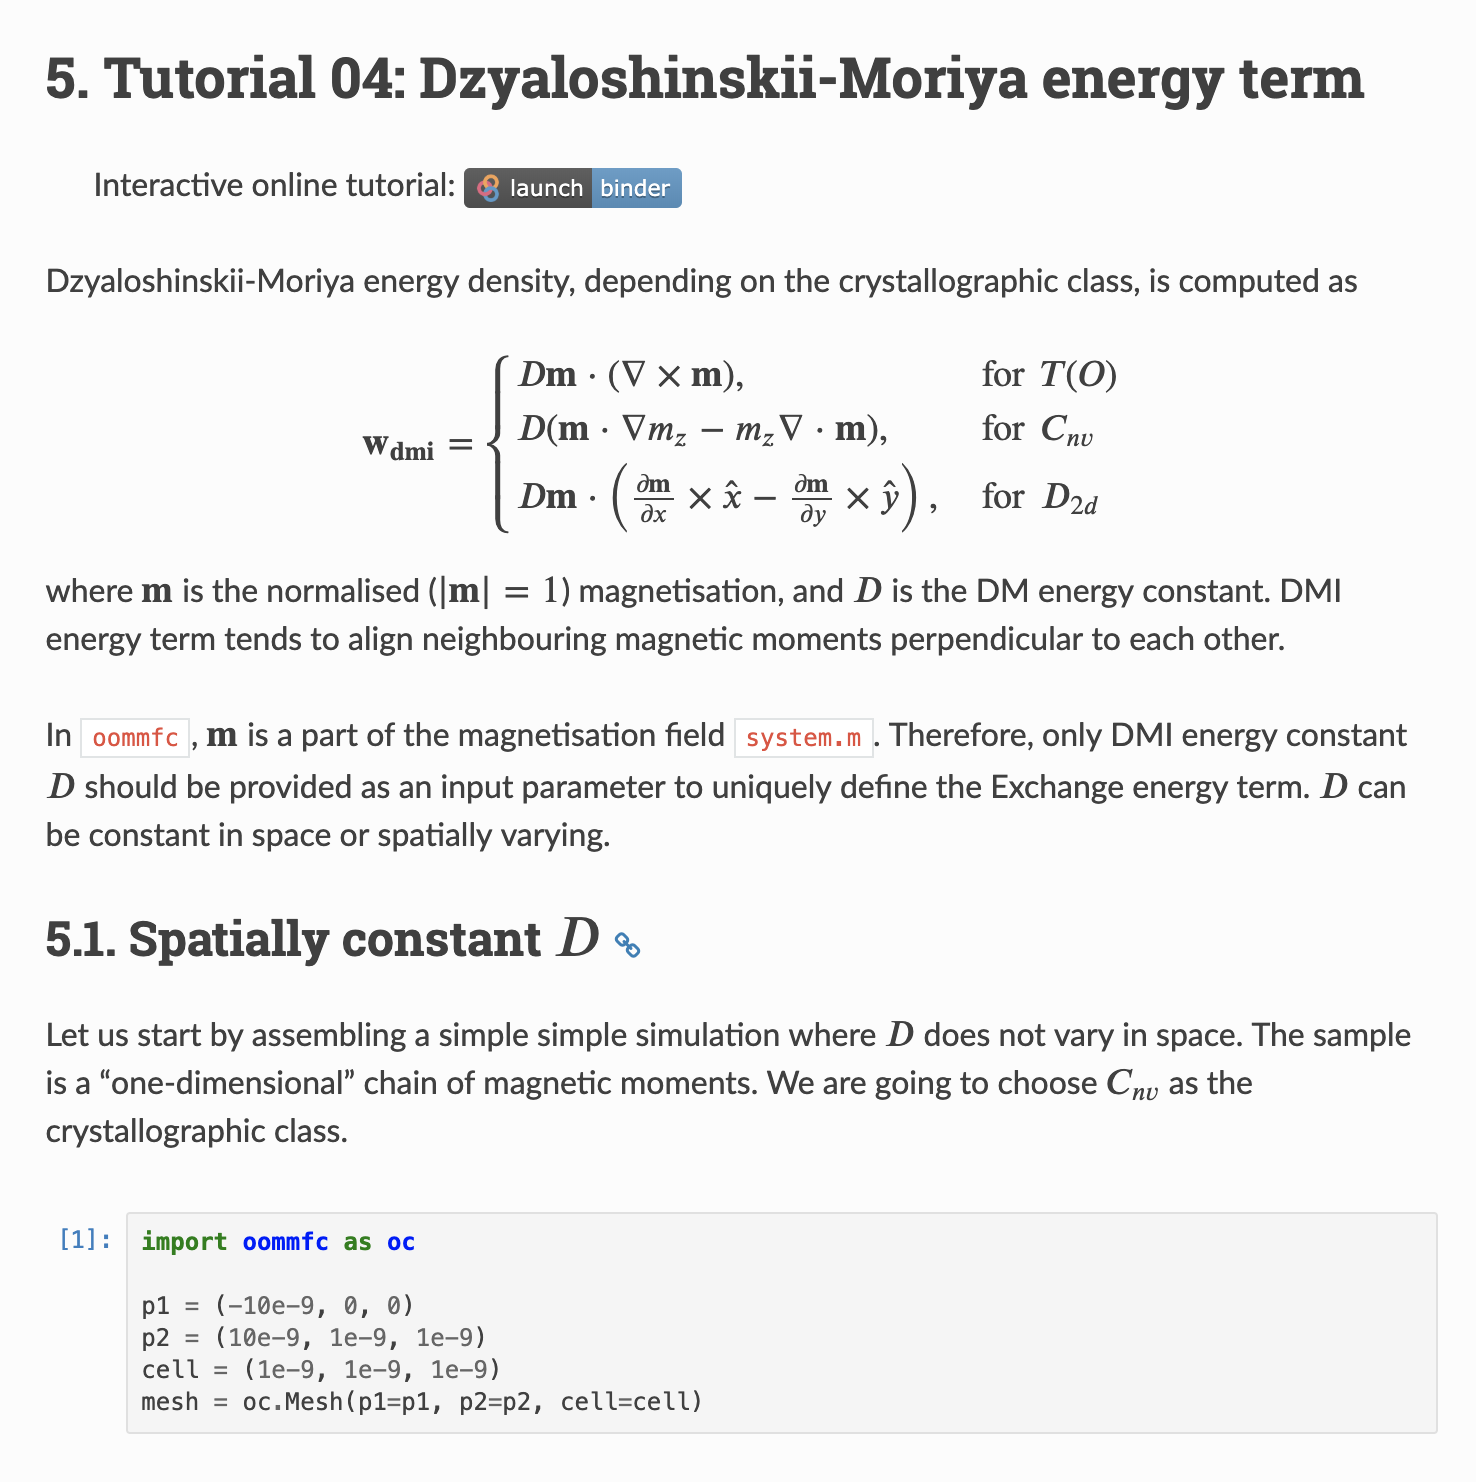
\includegraphics[width=1\textwidth]{demo1.png}}
  \caption{Figure showing the beginning of one of the micromagnetic
    notebook tutorials provided with Ubermag. At the top, there is the Binder
    badge which allows to execute this example interactively in the
    cloud. Below, markdown with integrated LaTeX equations is used to
    explain a particular type of nearest neighbour interaction that
    has recently received lots of attention. What follows in the
    notebook (not shown) is a physics simulation example that makes
    use of this interaction).  }
  \vspace*{2cm}
  \label{fig:demo1}
\end{figure}

\begin{figure}
  \centering
  \fbox{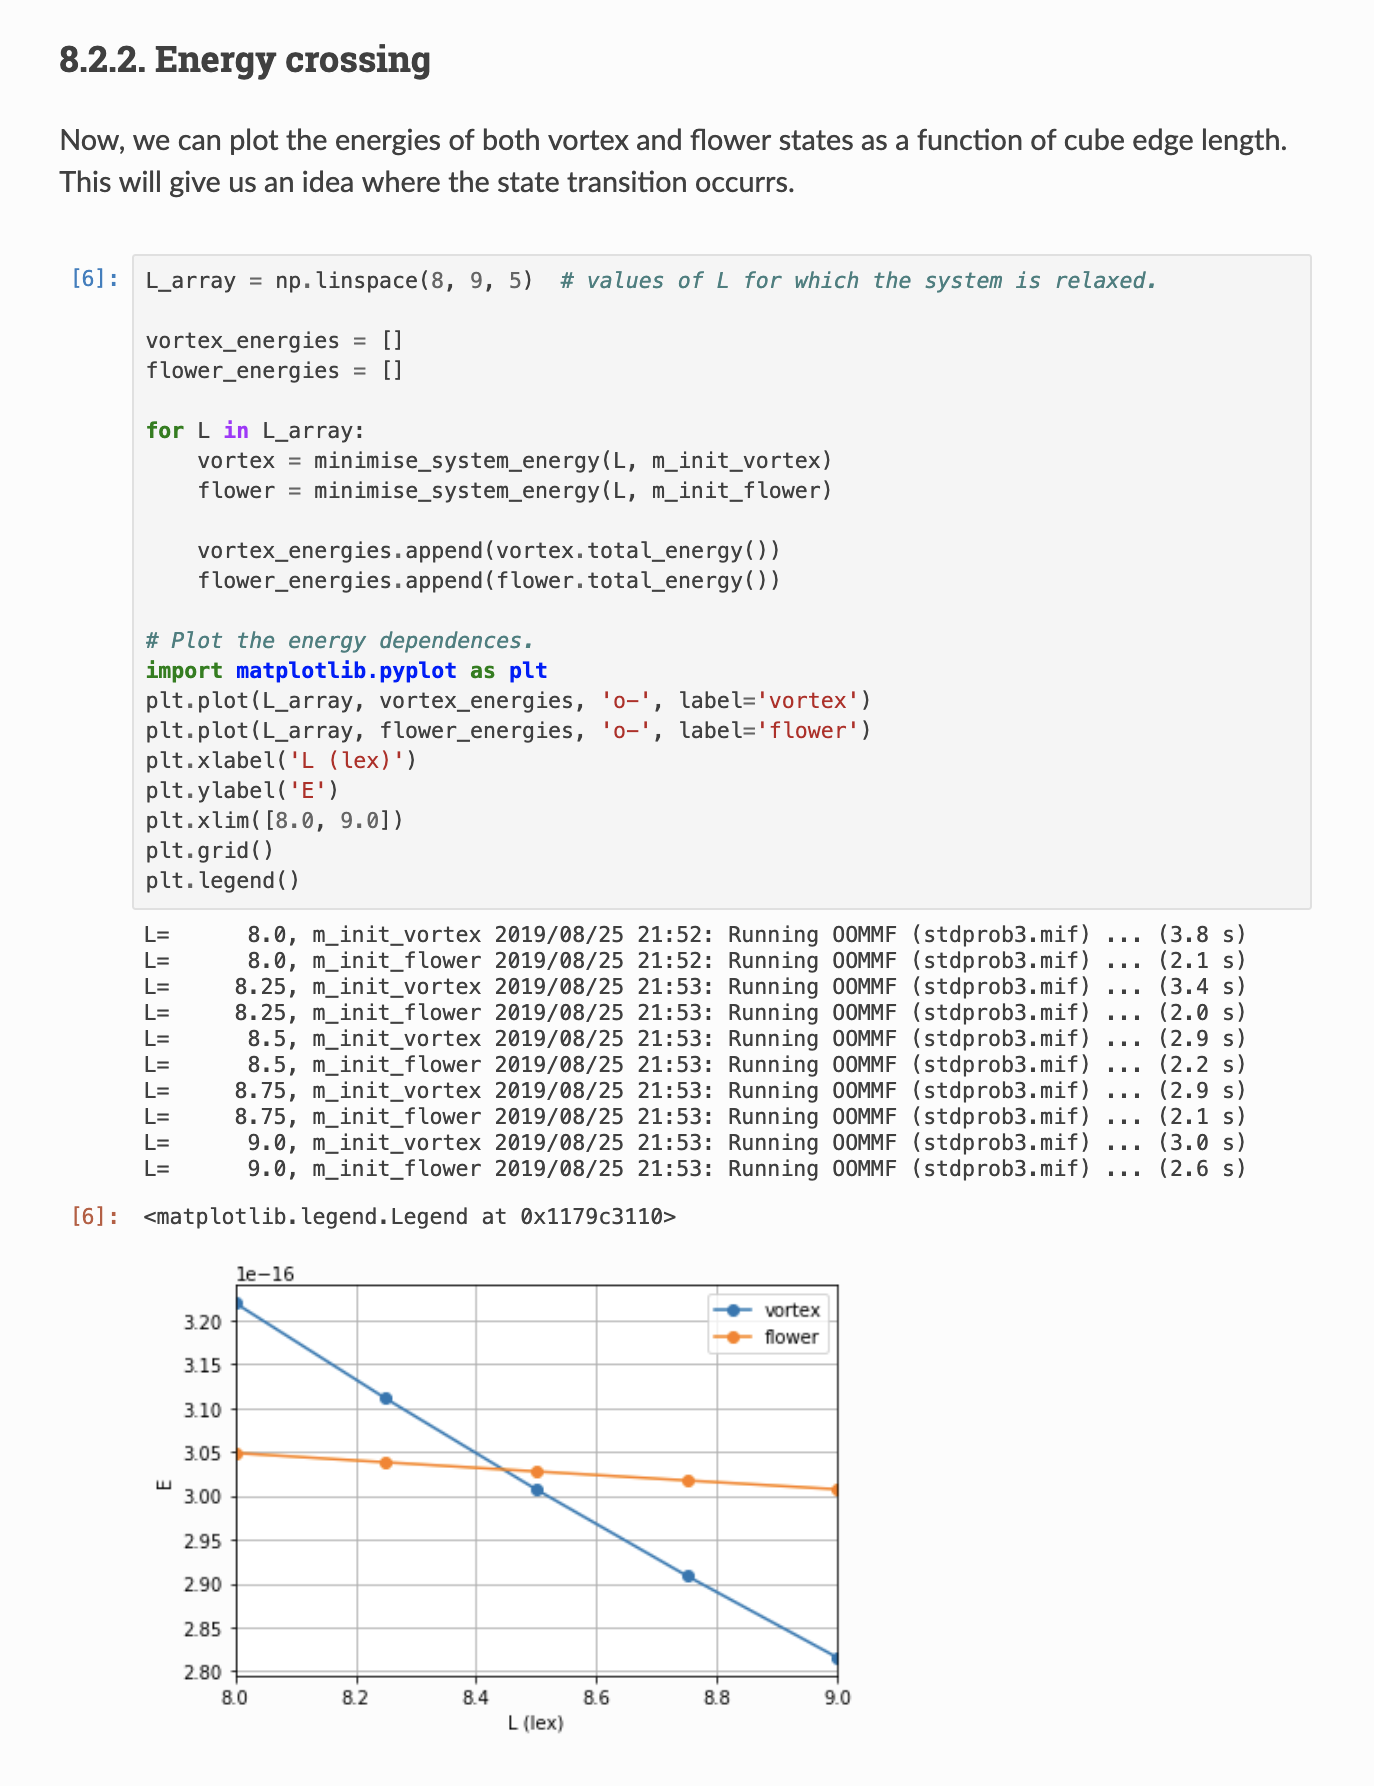
\includegraphics[width=0.95\textwidth]{demo2.png}}
  \caption{Figure showing a small part of one of the micromagnetic
    notebook tutorials provided with Ubermag. In this example recipe,
    we solve the well established micromagnetic standard problem 3.
    The integration of Ubermag commands with Python (i.e. the
    embedding of the micromagnetic domain specific language in Python \cite{Beg2017})
    allows to vary parameters (such as the parameter \texttt{L} in this
    example) through Python language constructs (such as a for loop),
    where previously these would have been done through bash
    scripting, and subsequent modification of OOMMF configuration
    files.  }
  \label{fig:demo2}
\end{figure}

\begin{figure}
  \centering
  \fbox{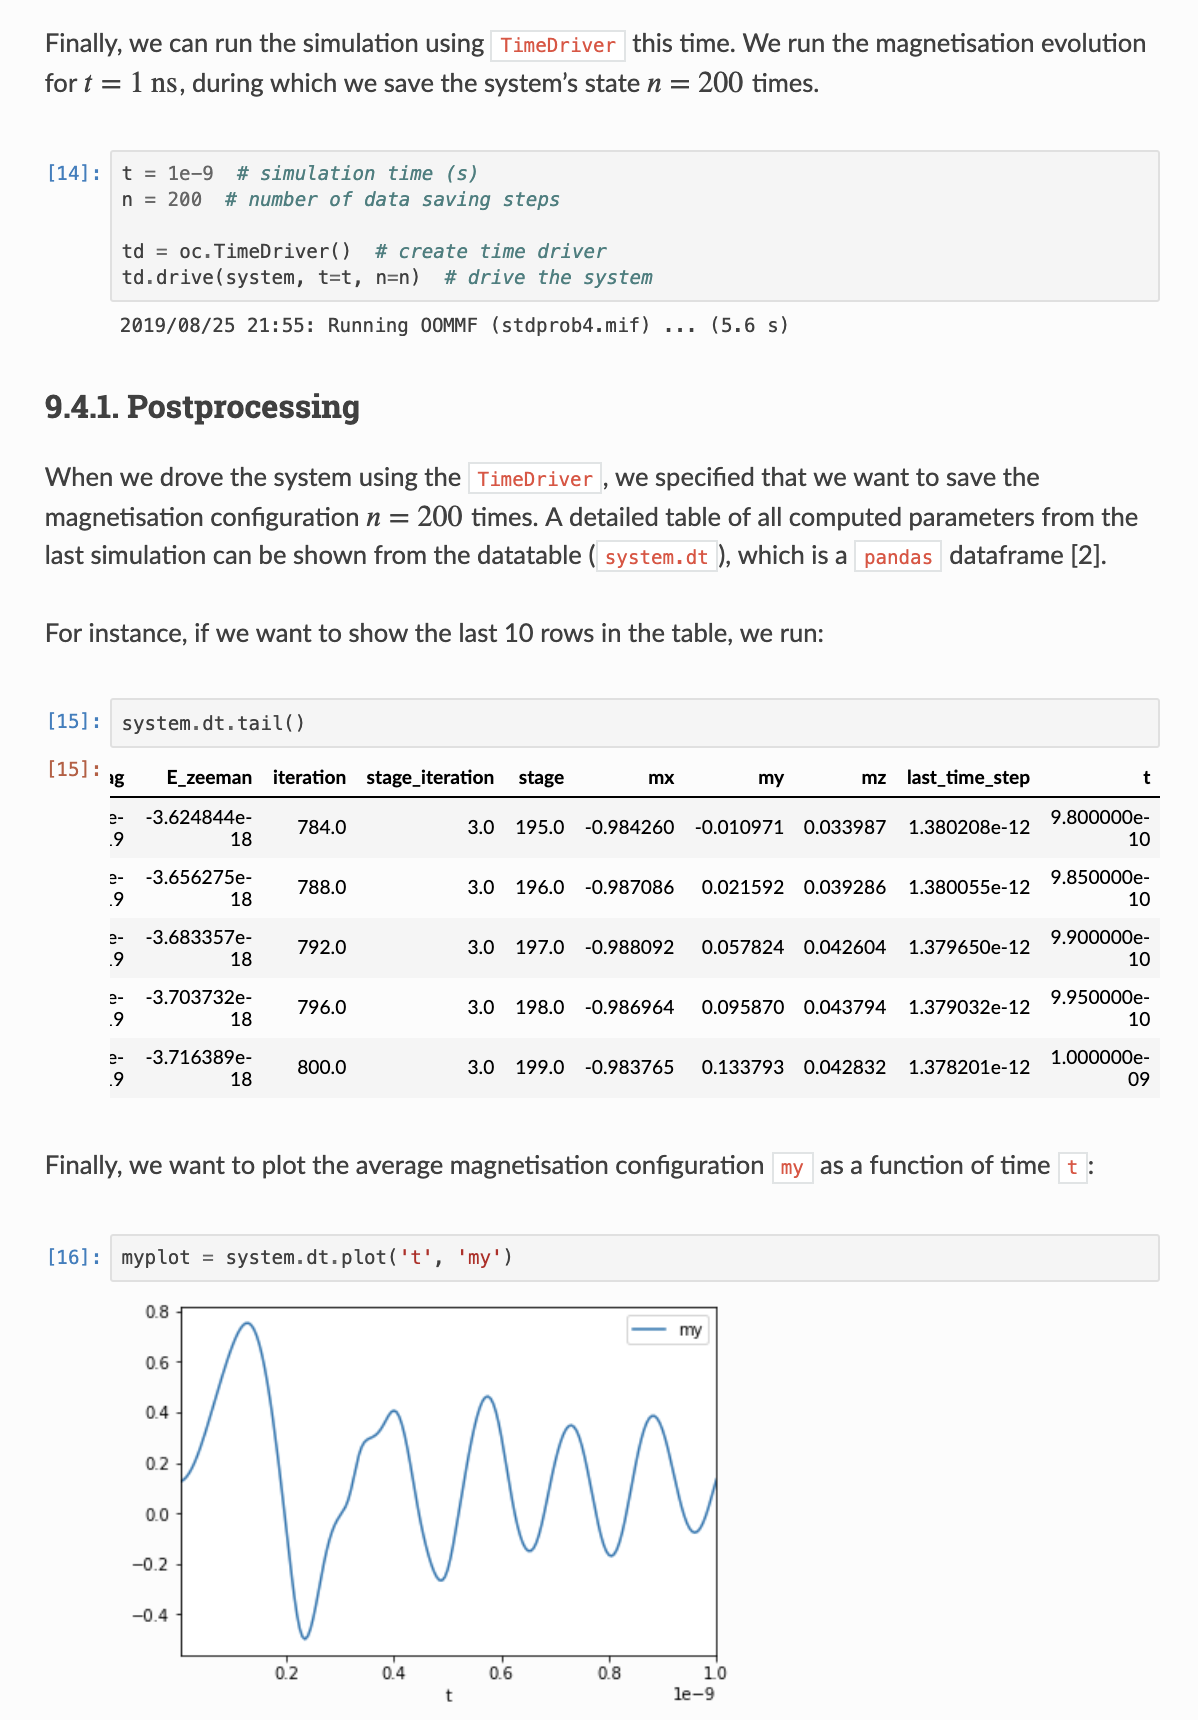
\includegraphics[width=0.92\textwidth]{demo3.png}}
  \caption{Figure showing part of the micromagnetic notebook tutorial
    for the micromagnetic standard problem 4: data that OOMMF is
    exporting into a tab-separated text file is automatically
    retrieved and made available in form of a pandas DataFrame. The
    creation of the plot (here plotting the column with data for time
    $t$ against the column with the y-component of the magnetisation
    $m_\mathrm{y}$) is a function of the DataFrame object.}
  \label{fig:demo3}
\end{figure}



\section{Implementation details}

The resulting package is called Ubermag and it is separated into
several different sub-packages:

\begin{itemize}
\item \texttt{discretisedfield}~\cite{discretisedfield} - reading,
  writing, analysis, and visualisation of scalar and vector
  fields. This package provides all the necessary functionality for
  reading resulting OOMMF vector and scalar field files and their
  analysis, such as sampling, iterating, computing averages and norms,
  and visualisation. For visualisation, we use two different
  approaches: (i) 2D visualisation of spacial slices of using
  \texttt{matplotlib} and (ii) 3D visualisation of both scalar and
  vector fields using \texttt{k3d}, which was developed as a part of
  \ODK as deliverable D4.12. The main benefit of this package is
  that all fields, after being created or read from files, are
  represented via \texttt{numpy} arrays, which enables exposing
  micromagnetic fields obtained from OOMMF to the Python scientific
  stack.
\item \texttt{ubermagtable}~\cite{ubermagtable} - reading and analysis
  of scalar table data. The main purpose of this package is to enable
  easy reading and analysis of OOMMF \texttt{.odt} files. This is
  achieved by converting the contents of an \texttt{.odt} file,
  created by OOMMF, to a \texttt{pandas} DataFrame object. Similar to
  exposing scalar and vector field data to Python's scientific stack
  in \texttt{discretisedfield}, in \texttt{ubermagtable}, this is
  achieved via \texttt{pandas} DataFrame, which enables easy analysis
  and visualisation of the table data, by exploiting the already
  existing infrastructure.
\item \texttt{ubermagutil}~\cite{ubermagutil} - typesystem used across all Ubermag
packages. This package contains the implementation of different Python
descriptors used for imposing a typesystem for individual attributes
in different classes.
\item \texttt{micromagneticmodel}~\cite{micromagneticmodel} - a domain
  specific language (DSL) for defining a micromagnetic
  simulation. Details about this package are explained in
  Sec.~\ref{sec:micromagneticmodel}.
\item \texttt{oommfc}~\cite{oommfc} - OOMMF calculator. After the
  micromagnetic simulation is defined using
  \texttt{micromagneticmodel}, \texttt{oommfc} translates the model
  into OOMMF simulation and runs it. Finally, all resulting simulation
  files are read by employing \texttt{discretisedfield} and
  \texttt{ubermagtable}. Details about this package are explained in
  Sec.~\ref{sec:oommfc}.
\item \texttt{micromagneticdata}~\cite{micromagneticdata} - data
  analysis convenience tools. This package contains code for the
  analysis of simulation results integrated in Jupyter notebook.
\end{itemize}

We decided to split the entire functionality of Ubermag into separate
smaller packages in order to allow users to use them individually. For
instance, \texttt{discretisedfield} package is a universal package -
not restricted to micromagnetics - and can be used for any
finite-difference field, such as in computational fluid dynamics.

\subsection{\texttt{micromagneticmodel}}\label{sec:micromagneticmodel}

The motivation for the development of the domain specific language
(DSL) for the definition of micromagnetic problems comes from the fact
that almost all micromagnetic problems can be defined in a unified
way. More precisely, in order to uniquely define a micromagnetic
problem, three main components must be defined:

\begin{enumerate}
\item \textbf{Initial magnetisation}. Magnetisation is a vector
field defined on a finite-difference mesh, so that one vector is
associated to each discretisation cell.
\item \textbf{Hamiltonian}. Depending on what energies are present in
the simulated sample, the Hamiltonian can contain different energy
terms. More precisely, the total energy of the system can be computed
as a sum of different energy terms computed for the particular
magnetisation configuration.
\item \textbf{Dynamics equation}. This equation governs the
magnetisation dynamics and, similar to Hamiltonian, it can contain
different dynamics terms.
\end{enumerate}

Because there is a uniform way how a micromagnetic problem can be
defined, we developed a domain specific language for defining such
problems. A model, defined using this domain specific language, is not
aware of the particular simulation tool that is going to perform the
actual micromagnetic simulation, but it is only used to describe the
problem.

\subsection{\texttt{oommfc}}\label{sec:oommfc}

The \texttt{micromagneticmodel} described in the previous section does not
contain any information on how the defined micromagnetic problem can
be translated into the OOMMF configuration file and run in
OOMMF. \texttt{oommfc} inherits all the functionality of
\texttt{micromagneticmodel} and specifies how all necessary elements
of the micromagnetic model can be translated into the OOMMF
configuration file. \texttt{oommfc} runs the simulation and after it
is completed, reads the resulting files and updates the system object.

\subsection{Open source code hosting and long term availability}

All the code developed as a part of this deliverable is hosted in
different repositories on the code hosting service GitHub as a part of
the Ubermag organisation. All the code is open source and publicly
available. In addition, snapshots of the repositories have been made
and all their contents are hosted in Zenodo.

\subsection{Automatic tests and continuous integration}

All individual packages of Ubermag are tested by running different
Python tests. There are three different types of tests:

\begin{itemize}
\item Direct testing of the source code. These tests are running
individual functionalities of different Ubermag packages as well as
larger micromagnetic simulations, such as standard problems. These
tests are also used for computing the code coverage - the percentage
of the code covered by tests.
\item Jupyter notebook tests. The majority of the Ubermag's
functionality is documented using Jupyter notebook. In order to make
sure that the documentation is up-to-date with the newest version of
the source code, they are tested using \texttt{nbval}, which was
developed as a part of OpenDreamKit deliverable
\delivref{UI}{jupyter-test}. More precisely, all individual code cells
in a Jupyter notebook are run and their results are compared to the
previous ones whenever a change is made in the source code.
\item API documentation tests. As a part of different class and
  function implementation, docstrings were included and later used for
  the API documentation. These strings usually contain small examples
  demonstrating the usage of individual features of the code. Similar
  to the testing of Jupyter notebooks used for documentation, we also
  test these docstring examples.
\end{itemize}

All three different types of tests are run on two different continuous
integration platforms: Travis CI for Linux and AppVeyor for Windows
operating system. These tests are triggered automatically each time a new commit to
the repository is made.

The codecov service is employed to record the
coverage of the tested code.

Latest continuous integration test results and code coverage links are
provided on the Readme page for every package.

\subsection{Documentation}

Each Ubermag package is individually
documented. There are two different types of documentation: (i) API
documentation, and (ii) examples of usage in Jupyter notebooks in the
form of tutorials and exercises.

API documentation, implemented via
docstrings, is generated by Sphinx. It contains the detailed
explanation of all possible ways of using different functions and
classes as well as small examples.

Jupyter notebooks provide tutorial-like documentation which explains
how different functionalities of a package can be used using
real-world problems to demonstrate this.

The top level documentation containing the tutorial on Ubermag, is a
part of \texttt{ubermag} meta-package. All the documentation is
generated as soon as a new commit is made to the repository and it is
hosted on readthedocs. In addition, several different tutorials, in
particular for the installation of Ubermag on different platforms, are
recorded as videos and hosted on YouTube.

All documentation can also be interactively used via Binder (a link
button is provided on every package's Readme file).

\subsection{Installation}

One of the main challenges scientists face in using simulation tools
is their installation. Contributing factors are that (i) research
software is generally not written by trained software engineers and
(ii) research software may require use of less commonly used libraries
which can be research products themselves, with associated behaviours
such as quickly changing interfaces, lack of support, lack of robust
installation procedures.

Therefore, we wanted to make the installation of Ubermag as simple as
possible.

All packages are built and made available for installation on
PyPI. However, installing Ubermag using pip is not going to install
OOMMF, which is a C++ code. Therefore, users have to install OOMMF
themselves and set the environment variable which points to the
installation path. Alternatively, Docker can be installed and before
the simulations are run, a Docker image will be pulled from Docker
cloud, container created, simulations run inside the container,
results extracted, and container destroyed. This approach allows the
maximum flexibility ion terms of the platforms allowed.

Alternatively, Ubermag can be installed via conda on all three major
operating systems (Windows, OSX, Linux). This approach installs not
only Ubermag, but also OOMMF. Detailed installation instructions are a
part of documentation and videos are created and hosted on YouTube.

\subsection{Ubermag in the cloud}

Apart from installing Ubermag on user's machine, Ubermag can be used
in the cloud. We provide this service using MyBinder where Jupyter
notebooks can be run on a temporary (container based) machine that is
provided in the cloud.

Running Ubermag in the cloud was particularly helpful when we
delivered workshops at various international conferences. More
precisely, due to the data protection rules, we were not allowed to
know the participants' information in advance so that we could contact
them and provide them installation instruction they should follow
before they arrive to the conference. Therefore, we had to deal with a
large number of simultaneous installations on different machines
before the workshop. This included downloading large installation
files, such as Anaconda and long waiting times for the installation to
complete. This can be counteracted by bringing mass storage media with
the required files available. Nevertheless, the amount of
configuration and fiddling with laptops with unusual behaviour (such
as: existing anaconda installation, lack of admin rights, outdated
hardware, lack of RAM, lack of disk space, ...) that was required to
enable all participants to actively take part in examples using their
own laptop, exceeded our resources.

Therefore, we asked all participants who were not able to
install Ubermag before the workshop to use Ubermag in the cloud, where
we hosted all materials we intended to cover during the workshop. All
they need for this is a web browser on their laptop.

\subsection{mumax3}

At the beginning of the project, our main focus was to develop a
Python interface to OOMMF and integrate it into Jupyter
notebook. After we developed a domain specific language in
\texttt{micromagneticmodel}, we decided to demonstrate its
universality for other micromagnetic packages. Therefore, we chose to
build another micromagnetic calculator for the
mumax3~\cite{Vansteenkiste2014} simulation tool. mumax3 is another
finite-difference package that is attracting increasing attention: its
main advantage is that it runs on GPU and it is usually much faster
than OOMMF. Accordingly, mumax3 is a simulation tool of choice when
the simulation speed is an important factor. In order to implement
another micromagnetic calculator, based on mumax3, we organised a
workshop at European XFEL and invited 5 participants. 3 participants
were from the research group at the University of Southampton, where
the OpenDreamKit project was previously hosted before moving to
European XFEL. Another 2 participants are the developers of mumax3
from the University of Ghent, Belgium. After a 4-day workshop we
managed to implement all the necessary functionality to run
micromagnetic standard problems using Ubermag and using mumax3 as the
computational backend.

\subsection{JOOMMF changes name to become Ubermag}

After the implementation of mumax3c, we decided to rename the entire
project from JOOMMF to Ubermag. The name ``JOOMMF'' originated from
Jupyter and OOMMF, but the new functionality is more general than
that.

This way, Ubermag provides the high level user interface which can
currently use two different micromagnetic calculators in the
background (i.e. OOMMF and mumax3).

There are some other finite difference packages that could be supported by
Ubermag in the future with modest effort.

\section{Dissemination}

During the project, we conducted several workshops at various
international conferences as part of our dissemination activities. At
these workshops we introduced the basics of micromagnetics and through
examples demonstrated how micromagnetic simulations can be performed
using Ubermag. All tutorials were followed by exercises which
participants could solve. The workshops we organised are:

\begin{enumerate}

\item DPG March Meeting, 19 March 2017, Dresden, Germany

  This meeting is the main annual conference organised by the German
  Physics Society. We were invited to contribute to the mini-symposium
  of the conference with the main topic micromagnetics. We had about
  50 attendees and we introduced the basics of micromagnetic
  simulations as well as the basics of running Ubermag. Unfortunately,
  the conference organisers did not allow us to have the details of
  participants or to take photos of the event due to the data
  protection regulations. This dissemination activity was fully funded
  by the OpenDreamKit grant.

\item Institute of Physics (IOP) Magnetism conference, 04 April 2017,
York, UK.

  This workshop was held together with Michael Donahue, NIST, USA, who
is the main developer and maintainer of OOMMF. In the first half of
the workshop, Michael Donahue introduced to the participants the
basics of micromagnetics as well as the main capabilities of the OOMMF
simulation tool. In the second half, we introduced a Python interface
to OOMMF by guiding the participants through several tutorials and
letting them to complete the exercises. We had approximately 30
participants at this workshop. Unfortunately, the conference
organisers did not allow us to have the details of participants or to
take photos of the event due to the data protection
regulations. Therefore, we had to ask the participants if they want to
provide us their information personally. This workshop was co-funded
with EPSRC CCP Computational Magnetism Network (EP/M022668/1).

\item Intermag 2017 conference, 24 April 2017, Dublin, Ireland

  This workshop was held at one of the major conferences in the field
of magnetism research. At the workshop we had 50 registered
participants, who had to register at the time of conference
registration. The maximum number of allowed participants was
determined by the conference organisers. The workshop was divided into
two parts: (i) main workshop event and (ii) follow up session. At the
main workshop event, we taught the participants the basics of
micromagnetics and how they can use Ubermag in their every-day
research. In the follow-up session, we talked to the participants of
the main workshop event as well as to those who wanted to attend, but
who could not register due to the limited number of spaces. In the
follow-up session we were able to discuss the Ubermag capabilities in
more detail as well as to answer any specialised questions current or
potential users might have. In both sessions we were able to receive
some feedback and feature requests from users, as well as addressing
their questions. This workshop was
co-funded with EPSRC CCP Computational Magnetism Network
(EP/M022668/1).

\item 62nd Annual Conference on Magnetism and Magnetic Materials, 6-10
Nov 2017, Pittsburgh, PA, USA

    Similar to Intermag, this is one of the major conferences in the
field of magnetism research. We were not able to organise the workshop
jointly with the conference organisers. Therefore, we organised an
informal workshop at the conference, comparable to a drop-in or
ask-the-expert session. We invited all
interested participants to come and see us at the conference using
several micromagnetics oriented mailing lists. At the workshop we had
both Ubermag users and researchers who could potentially start using
Ubermag. We were able to introduce to all interested participants the
main capabilities of OOMMF as well as the benefits of using our Python
interface and Jupyter integration.

\item Advances in Magnetism 2017 conference, 04-07 February 2018, La Thuile,
Italy

    This event was organised as a tutorial session for all conference
attendees by the conference organisers. This was structured as an
invited talk. During the 30 min talk we explained the basics of
micromagnetics as well as the benefits of Ubermag. In addition, we
provided enough information for the participants to start using
Ubermag on their own. At this event, we had more than 100
participants.

\item International Conference on Magnetism, 14-20 July 2018, San
Francisco, USA

    This workshop was a part of the official conference
    programme. Jointly with the conference organisers, we organised a
    workshop which was offered to all conference participants. No
    limitation on the number of available places was imposed by the
    organisers. The conference attendees were offered to register for
    the workshop at the time of conference registration. Similar to
    the the previous events, we were not allowed have the details of
    the participants. At the workshop, we had more than 70
    participants. At the workshop we had both Ubermag users and
    researchers who could potentially start using Ubermag. The
    workshop was divided into two parts: (i) main workshop event and
    (ii) follow up session. At the main workshop event, we taught the
    participants the basics of micromagnetics and how they can use
    Ubermag in their every-day research. In the follow-up session, we
    talked to the participants of the main workshop event as well as
    to those who were not able to attend on the first day of the
    conference. In the follow-up session we were able to discuss the
    Ubermag capabilities in more detail as well as to answer any
    specialised questions current or potential users might have. In
    Fig.~\ref{fig:icm-workshop} we show the photo taken at the
    workshop.

    \begin{figure}
      \includegraphics[scale=0.3]{IMGP7466.jpg}
  \caption{\label{fig:icm-workshop} Computational micromagnetics with
    JOOMMF workshop at the International Conference on Magnetism,
    14-20 July 2018, San Francisco, USA}
    \end{figure}

\item Joint Magnetism and Magnetic Materials - Intermag conference,
14-18 Jan 2019, Washington DC, USA

    Similar to other MMM conferences, we could not organise the
workshop jointly with the conference organisers. Therefore, we invited
all interested participants to come and see us at the conference using
several micromagnetics oriented mailing lists. At the workshop we had
both Ubermag users and researchers who could potentially start using
Ubermag. We were able to introduce to all interested participants the
main capabilities of OOMMF as well as the benefits of using our Python
interface and Jupyter integration. As before, we received valuable
feedback from the participants.

\end{enumerate}

Due to the restrictions imposed by the conference organisers, we were
not able to take photos and get personal information from the
participants. Therefore, we asked them to voluntarily do our online
survey.

In addition to the workshops listed above, we have delivered some conference
talks on Ubermag (which was called JOOMMF at the time) addressing 3
different audience groups:
\begin{itemize}
\item Hans Fangohr: A case study of computational science in Jupyter
  notebooks: JOOMMF, Computational Mathematics with Jupyter Workshop,
  Edinburgh (UK), 20 Jan 2017
\item Hans Fangohr: User interfaces for computational science: a
  domain specific language for OOMMF embedded in Python , Magnetism
  and Magnetic Materials Conference, New Orleans, Louisiana (US), 2
  Nov 2016
\item Hans Fangohr: Driving Simulation and Data analysis of magnetic
  nanostructures through Jupyter notebooks. PyCon.DE 2018, Karlsruhe,
  (Germany), 24 October 2018
\end{itemize}

A publication on the micromagnetic abstraction of Ubermag is
available: Marijan Beg, Ryan A. Pepper, Hans Fangohr. \emph{User interfaces for
  computational science: a domain specific language for OOMMF embedded
  in Python}, AIP Advances 7, 056025 (2017), https://doi.org/10.1063/1.4977225

\section{Evaluation}

We evaluated Ubermag by asking users as well as the participants at
different workshops to complete our online survey. Basic conclusions
about our users/participants and their previous experiences we got
from the survey are:

\begin{itemize}
  \item The majority of our users/participants are students (56.1\%),
whereas 43.9\% of them are employed. Similarly, the vast majority of
them are employed in academia (90.2\%) - much more than in industry
and government laboratories. The age of our participants is 18-34 (78\%) and
35-54 (22\%).
\item Firstly, we asked both current and potential Ubermag users
whether they are active in the field of magnetism research. 92.7\% of
participants answered they are. However, from another question if they
have ever performed a micromagnetic simulation 65.9\% of participants
answered that they have not. Accordingly, we concluded that the
majority of participants at our workshops had no previous experience
of running micromagnetic simulations and they attended our workshops
not only to learn a new simulation tool, but to learn general
micromagnetic simulation techniques. After we learned this
information, we restructured our future workshops and taught users for
the first half of the workshop the basics of micromagnetics. In the
second half of the workshop we focused on Ubermag.
\item For those participants, who have performed micromagnetic
simulations before, we asked them what simulation tool they have
used. More than two thirds answered that they have used or are
actively using OOMMF. This confirmed our initial prediction that OOMMF
is the most widely used simulation tool at the moment of the project
proposal. In the second place (37.5\%) was mumax3, which is reflects
our decision to demonstrate the universality of our domain
based language for the description of micromagnetic problems by adding
mumax3 as another computational back-end.
\item We wanted to know what computational science tools they
have used in the past and how familiar they are with the state-of-the
art tools we used to develop our Python interface to OOMMF. The
majority (more than two thirds - 68.3\%) of users are working on
Windows operating system. In the second place was MacOS (31.7\%) and
Linux (24.4\%). These results confirmed our idea of making the
installation simple on all three major operating systems by building
conda packages. All participants have heard previously about Python
and 70.7\% of them have used it before. However, 60\% of all
participants do not have enough experience in using Python and
consider themselves to be beginners. Only 12.2\% of users think they are
advanced users of Python. These findings confirmed several of our
observations at the workshops. Although we built a a much simpler to
use interface to OOMMF and integrated it into Jupyter notebook, for
new users learning Ubermag is still a steep learning curve. This is
partly because they are new to Python, but mostly due to the fact that
they have no prior programming experience.
\item In terms of Jupyter notebooks, 63.2\% of our participants have
heard about the Jupyter notebook, but only 26.8\% are actively using
it. On the other hand, 36.6\% of users have never heard of it.
\item The questions regarding the use of more advanced tools in
computational science, such as Docker and Anaconda, the vast majority
have never heard of it.
  \item We asked users to give us an overview of what expectation do
they have from a new simulation tool they want to employ in their
every-day research. In the first place is the ease of use, which
confirmed our initial predictions that it is necessary to have a
simple, intuitive, and understandable user interface. This was what
guided us in the development of Ubermag. Secondly, simple installation
was marked as a second most important factor. This, in combination
with the computational habits of our users motivated us to make a
simple installation procedure based on Anaconda. Last but not least,
documentation, visualisation capabilities, and speed were mentioned
and some of the factors users consider before they decide to use a
micromagnetic simulation tool.
\end{itemize}

In addition to general questions we asked users about their previous
experiences in computational science and micromagnetics, we asked
users to give a direct feedback on what they like and do not like
about Ubermag. The vast majority of participants answered that they
think Ubermag is user friendly and simple to use. Among the things
they do not like, they say that documentation was not complete which
comes from the fact that most of the workshops were held early on in
the project and not all documentation was complete at that
point. Secondly, users complained about the installation due to
certain limitations they experienced on their machines.

\section{Administration}

\subsection{Move from the University of Southampton to European XFEL}

The OpenDreamKit project with principal investigator Hans Fangohr and
postdoctoral researcher Marijan Beg moved from the University of
Southampton (UK) to European XFEL (Germany) on 1st September 2017. The
last day of OpenDreamKit at the University of Southampton was 31st
August 2017. The move was initiated by the offer and acceptance of a
new position for Hans Fangohr at European XFEL. There were no problems
encountered in the relocation process. The facilities at European XFEL
are suitable for the completion of OpenDreamKit and the administrative
support is provided. Tasks started at Southampton will be continued at
European XFEL. There are no parts of OpenDreamKit left at the
University of Southampton.

\subsection{Sergii Mamedov}

In addition to Marijan Beg, who was fully employed on the OpenDreamKit
project, between Oct 2.18 and February 2019 Sergii Mamedov was
employed. The reported work contains additional contributions from
Ryan Pepper and Thomas Kluyver.

\section{Summary}

Above, we have summarised the creation of the Ubermag micromagnetic
simulation environment. Although we know of some publications that
make use of Ubermag (at the time it was still called JOOMMF), such as
 \cite{Cortes2018}, \cite{Gilbert2019} and \cite{Kannan2019}, it is too
early to comment on uptake of this technology/tool in the community.

From interactions with users we have seen, however, that the model of
directing and coordinating computational science studies from inside
the Jupyter Notebook environment is popular with scientists - a key
feature is the integration of code (i.e. the detailed and exact
description of the computational process) with the outcome in one
document. Another import point is that the people doing the technical
work can convert the notebook to html or pdf and send it/show it to
collaborators and supervisors who can then enjoy the document
including its multimedia components within their webbrowser (but
importantly without having to install software).

The integration of elements similar to graphical user interfaces (that
can be realised with ipywidgets) has also been welcomed and allows
blending of command driven and GUI-supported data analysis.

Another item of feedback from interactions with power users and
decision makers in computational science projects was that the
creation and maintenance of nbdime and nbval was highly welcome and
allows to use Notebook-driven projects more effectively.

A technical difficulty we encountered is that some packages
(IPywidgets, k3d) do not work reliably for all major browsers for both
the classic Jupyter Notebook and the next generation JupyterLab. This
is maybe not unexpected given the high rate of change in these
community driven projects but affects robustness of tools based on
these infrastructures. However, we expect these difficulties to
improve as those packages mature and the transition from Jupyter to
JupyterLab is complete.

For completeness, we'd like to mention that during this work, we have
become aware of a related initiative\cite{ase-paper} that provides an
\emph{atomic simulation environment} and provides a high level user
interface to a number of atomic simulation tools, similar to the way
that Ubermag provides a high level user interface to some
micromagnetic tools.

Looking beyond the area of micromagnetism, we can see that the model
of virtual research environments based on the Jupyter project and
developed and demonstrated here have already affected the provision of
data analysis software environments, for example at the European X-ray
Free Electron Laser facility in Germany and its partners in the PaNOSC
project\footnote{Photon And Neutron Open Science Cloud, EC research
  and innovation programme grant agreement No 823852,
  http://panosc.eu}, which we expect to also feature in (parts of) the
European Open Science Cloud user interface and capabilities.

\newpage\printbibliography

\end{document}

%%% Local Variables:
%%% mode: latex
%%% TeX-master: t
%%% End:
